% Activate the following line by filling in the right side. If for example the name of the root file is Main.tex, write
% "...root = Main.tex" if the chapter file is in the same directory, and "...root = ../Main.tex" if the chapter is in a subdirectory.
 
%!TEX root =  ../Thesis.tex

\chapter[ATLAS Detector]{CERN, the LHC Accelerator and the ATLAS Detector}




\section{Introduction}
Experimental particle physics research has many prominent features, but the most prominent
might be the scope and collaborative nature of the work.  This thesis is one of many that have
been produced at the ATLAS dectector at CERN, and makes use of the dedicated work of many
physicists to build and maintain the experimental apparatus and data processing pipeline.
The Large Hadron Collider is the first major piece of this, where beams of protons are accelerated to
tremendous energies and the smashed into each other inside the cavernous detectors, including ATLAS.
It is the collisions
between individual pairs of protons that underpin the entire scientific mission: in this environment,
interesting and rare physics can result from the interactions between the protons.  It is the mission of the
LHC to generate large numbers of high-energy proton-proton collisions, and then the mission of the detectors
to record and analyze the data that results from the collisions.  



%http://home.web.cern.ch/about/accelerators
\section{CERN and the Large Hadron Collider}
\label{sec:cern_lhc}
The European Center for Nuclear Research (CERN) is a scientific complex in Geneva, Switzerland that was established 
in the years following World War II.  Its focus is experimental particle physics, in particular the Large Hadron 
Collider (LHC), and it has a long and storied history of producing particle discoveries and other scientific
advances.

The LHC is the particle accelerator that serves as the centerpiece of CERN's scientific program.  The accelerator is 
an RF-driven circular sychrotron located in an underground tunnel with a circumference of 27 km, and when 
it is running, accelerates and collides two proton beams (sometimes two lead ion beams, but we will 
focus on the protons in this thesis) at four interaction points around the accelerator ring.  Each of proton beam 
contains thousands of bunches of protons which are very deliberately spaced so that every 50 ns, two 
of those bunches going opposite directions will overlap at one of the interaction points.  In 2012, the energy
of the proton beams was 4 TeV each, making for a total of 8 TeV of energy when the beams are collided head-on.
These are the highest-energy proton-proton collisions ever created by man-made acceleration, and reliably making lots of
collisions is a scientific and engineering endeavor completely in its own right, even before considering
the physics insights that we get as a result.


There are two major figures of merit for any particle accelerator: energy and luminosity.  Energy is typically limited 
by the circumference of the accelerator and by the magnetic field strength of the accelerator's bending magnets.  
The record-breaking energy of the LHC is a function of its tremendous size (27 km in circumference) as 
well as 1232 8.4 tesla superconducting dipole magnets that keep the beams in place within the accelerator.  Luminosity 
 is a measure of how many collisions the accelerator can produce, with higher luminosities meaning that more 
interesting events (and non-interesting events!) can be generated.  Since different processes happen at different rates
, the rate at which a given process occurs is usually stated in terms of its production cross section.  
Cross sections are measured in units of barns (or fractions thereof), with one barn being equal to 10
$^{-28}$ $m^2$.  Luminosity is measured in inverse barns, so that he cross section 
can be multiplied by the luminosity to give a total number of events for that type of event.  Luminosity 
is usually limited by the intensity and focus of the beam, and the bunch crossing rate.


%http://inspirehep.net/record/805147/plots
\begin{figure}
	\centering
	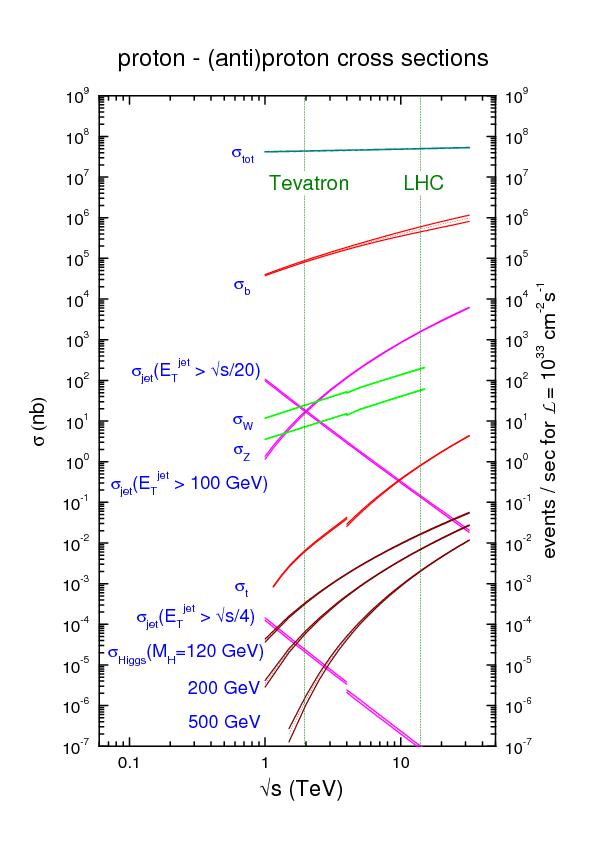
\includegraphics[width=0.6\textwidth]{ATLASDetector/images/crosssections2008.png}
	\caption{Cross sections for various processes as a function of center-of-mass energy
            of the original collision.  The ``skip'' at 4 TeV occurs because below that
            value, the cross sections are for proton-antiproton collisions like those
            made at the Tevatron, while higher energy collisions are being produced
            at the LHC. \label{fig:cross_sections}}
\end{figure}


Energy and luminosity go hand-in-hand to push back the frontiers of physics.  One of the 
major goals of the LHC is to discover new particles, and by conservation of energy the higher the LHC 
can go in energy, the heavier it can go in new particles to potentially create.  Another important fact 
is that, while cross sections for all types of processes typically go up as the collision energy increases, 
many new physics models have production cross sections that go up faster than the backgrounds as a function of center
-of-mass energy.  In other words, for a given process, the signal-to-
background ratio tends to go up as energy increases so new physics can be much easier to spot at higher 
energies than at lower energies.   

Discovery reach can also be extended by increasing the luminosity of a machine, 
since sensitivity to a signal is typically defined as $s/\sqrt{b}$--for example, a 
10-fold increase in luminosity means a $\sqrt{10}$-fold increase in a search's sensitivity.  
Luminosity can be increased by either tuning the accelerator to have a higher instantaneous luminosity, with a more focused 
beam or higher beam current for example, or by simply running the machine for a longer time.  In 
practice, increasing instantaneous luminosity at the LHC also means increasing the number of lower
-energy collisions that, while not of physical interest, still get picked up in the detector (pileup
).  The removal of pileup is an intense and dedicated effort that will be addressed in Section~\ref{sec:pileup}.



%%% lumi in 2010, 2011 and 2012
\begin{figure}
	\centering
	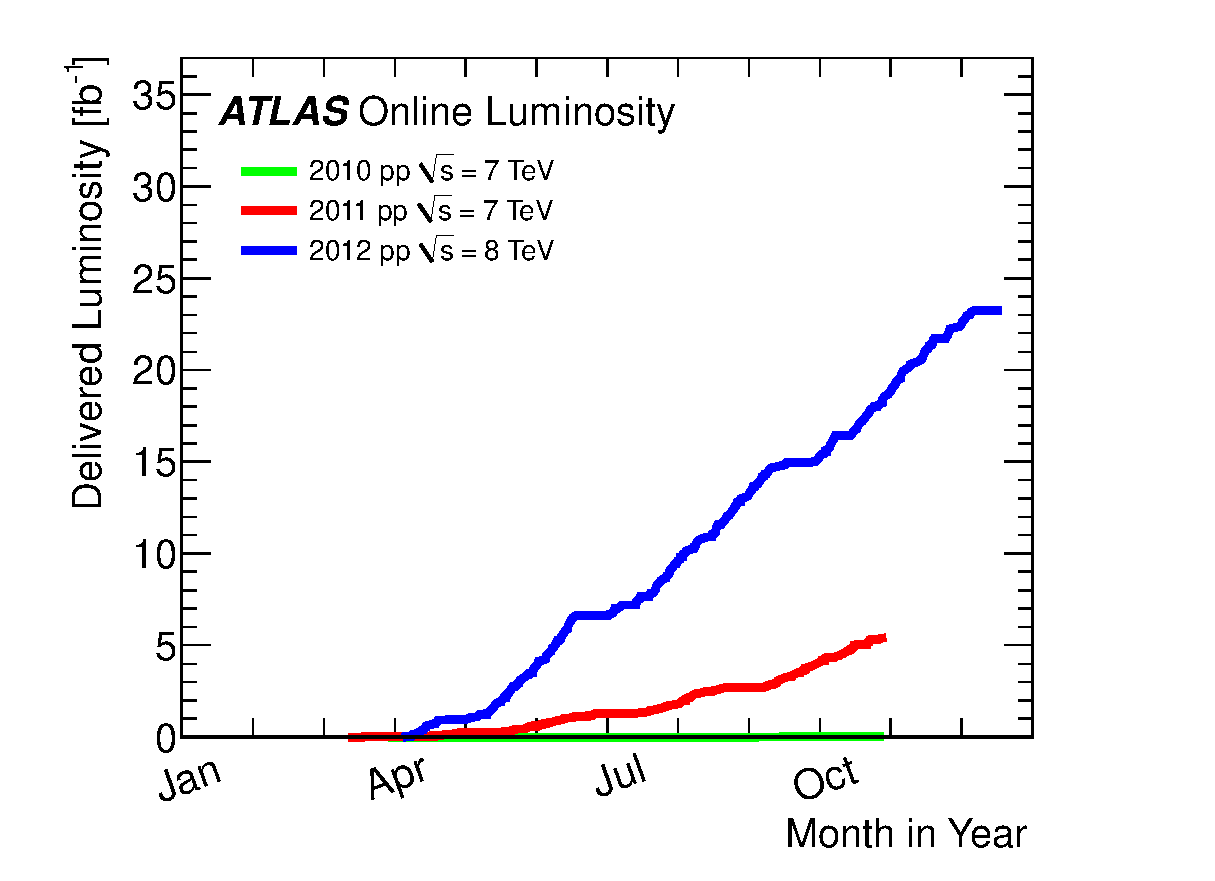
\includegraphics[width=0.6\textwidth]{ATLASDetector/images/intlumivsyear.eps}
	\caption{The luminosity collected in 2010, 2011 and 2012 at ATLAS. \label{fig:lumi_vs_year}}
\end{figure}



The LHC is only the last in a chain of accelerators, which all work together to create the high 
energy and luminosity that we associate with the LHC.  The first step in the process is the proton source
, where hydrogen atoms are subjected to an electric field that separates the protons from the electrons.  Then the 
protons are accelerated by a 90kV field and focused, and fed into a linear accelerator.  From this point 
forward, all the accelerators use radio frequency (RF) electromagnetic waves to impart energy to the protons.  

The linear accelerator brings the protons up to an energy of 50 MeV, then they go to the Proton 
Synchrotron Booster (up to 1.4 GeV), and then the Proton Synchrotron (25 GeV).  Then 
the protons are passed to the Super Proton Synchrotron, where they reach an energy of 450 GeV, and 
finally the beam is split into half and each half is injected into the LHC going a different direction.  
Figure ~\ref{fig:accelerator_complex} shows all the major accelerators at the CERN site.



%%% CERN accelerator figure
\begin{figure}
	\centering
	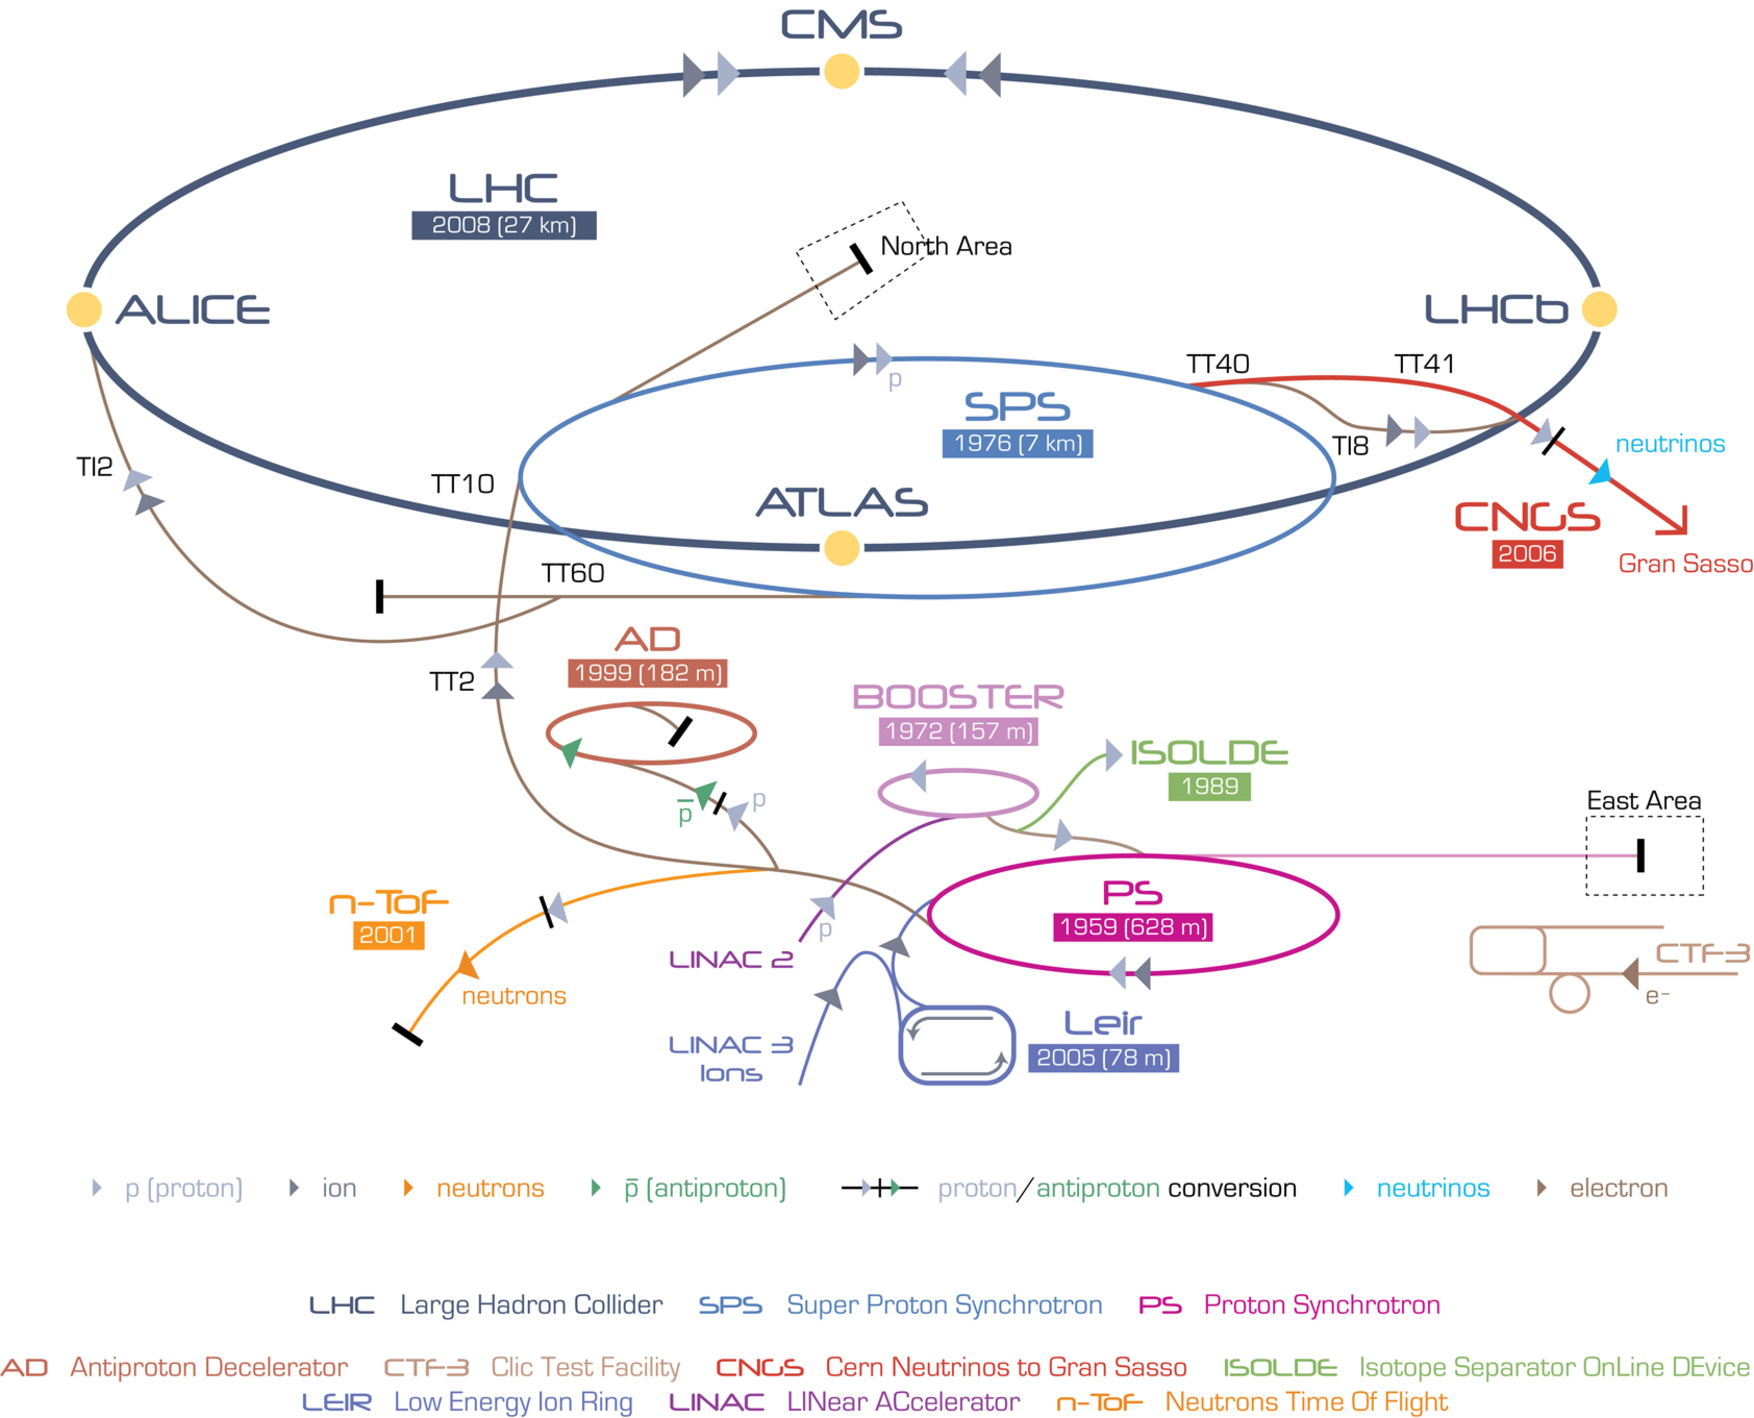
\includegraphics[width=0.8\textwidth]{ATLASDetector/images/Cern-Accelerator-Complex.pdf}
	\caption{ The major elements in CERN's accelerator complex, which turns ordinary hydrogen atoms in the highest-energy man-made collisions ever made. The four interaction points, labeled for their respective experiments (ALICE, ATLAS, LHCb and CMS) can be seen around the perimeter of the LHC. \label{fig:accelerator_complex}}
\end{figure}



Once the beams are in the LHC, they are accelerated up to the full collision energy of 4 TeV 
per beam.  Then the beams are focused  and carefully steered into position so that head-on collisions commence
.  The protons are arranged in bunches within the beams, with each bunch 50 ns away from its neighbors
, so that the collision frequency within the detectors is 20 MHz.  The data-taking is organized into 
runs, where collisions are created continuously for up to 16 or so hours at a time.  A run 
typically ends either when enough of the beam gets burned away by the collisions that the instantaneous luminosity drops and 
it becomes worthwhile to refill, or when a technical glitch causes the beams to be dumped.

The history of the LHC is a dramatic one.  The LHC first turned on in 2008, but within 
days had to shut down following a catastrophic failure of the bus bar between superconducting magnets.  It restarted in 
2009 at 7 TeV, half the design energy of 14 TeV (a repercussion of the accident), and 
the first run for physics was performed in 2010, with a total dataset size of 36 inverse picobarns.  
The progress in 2011 was dramatic, as the beam intensity was steadily increased over the course of the run 
to create an exponential increase of the luminosity recorded, and at the end of 2011 the total dataset size 
was about 5 inverse femtobarns (a factor of more than 1000 greater than the data recorded in 2010).  
The progress continued in 2012, with a slightly increased energy of 8 TeV and about 20 $fb^{-1}$ 
collected, culminating in the 4 July 2012 announcement of the discovery of a new particle, later confirmed to 
be the long-sought Higgs boson.  The total collected luminosity is illustrated in Figure~\ref{fig:lumi_vs_year}.  
At the end of 2012, the LHC commenced a 2-year shutdown to complete upgrades and repairs, 
with the intention of starting up again in 2015 at 13 TeV and 25 ns spacing between bunch crossings.
When the LHC starts up again, the search for new particles will begin again as both energy and luminosity
records are broken by the upgraded machine.



\section{The ATLAS Coordinate System}
The ATLAS detector is situated at Point 1 of the LHC ring.  Since the detector has a cylindrical shape
, polar coordinates are the most natural basis for describing its geometry.  The radial direction (usually notated ``r'') 
is defined as the vector originating at the interaction point, in the middle of the detector, and pointing 
transverse to the beamline.  The azimuthal angle $\phi$ and the polar angle $\theta$ complete the 
coordinate system, although in practice it is more common to use pseudorapidity $\eta$ instead of $\theta$.  
Pseudorapidity has the advantage of being a quantity that is Lorentz-invariant under boosts longitudinal to the incoming beams 
(in a hadron collider, the longitudinal component of the momentum of the incoming partons is not known).  
The definition of pseudorapidity $\eta$ is

\begin{equation}
\eta = -ln(tan( \frac{\theta}{2} ))
\end{equation}

Since the proton is a composite particle, made of three valence quarks and an indeterminate number of gluons, even 
if the proton has a known energy, its constituent partons can have a wide range of energies.  In 
general, then, the exact collision energy can vary from event to event, and outgoing particles can be 
boosted forward in $\eta$.  However, energy is conserved in the $\phi$ dimension, so transverse 
energy and momentum ($E_T$ and $p_T$, respectively) should add up to zero in events where there are no particles escaping detection.

\section{The ATLAS Detector}
The ATLAS detector is like an onion: it has layers, and it makes you cry.  There are 
several main subsystems, each of which is designed to measure a certain characteristic (charge, momentum, energy
, etc.) of a particular type of particle (quark, electron, muon, etc.).  The subsystems 
work hand-in-hand with the trigger and data acquisition system, which handles the decision-making 
of which events to record and goes about writing those events to disk.  

\subsection{Inner Detector}
The innermost layer of the ATLAS detector is the tracker, which provides precision measurements of the trajectories of charged 
particles.  As a charged particle traverses the layers of the tracker, it ionizes the detector material which creates 
small electrical signals that can be amplified and read out by the system.  These so-called ``hits'' 
are combined during reconstruction into tracks, which represent the paths of particles like electrons, muons, and charged 
pions in the detector.

The information from the tracker is used in particular to determine the transverse momentum (p$_T$) of 
charged particles, and to perform particle identification.  The tracker consists of three primary subsystems: the pixels, 
semiconductor tracker (SCT), and transition radiation tracker (TRT).  A charged particle created at or near the 
interaction point would typically travel through all three subsystems, creating some number of hits in each one.  On 
average, a track has 3 pixel hits, 8 hits in the SCT (4 double-sided hits
) and about 34 hits in the TRT, with all the inner detector subsystems enclosed by a 2 tesla solenoidal magnetic field. 


\begin{figure}
	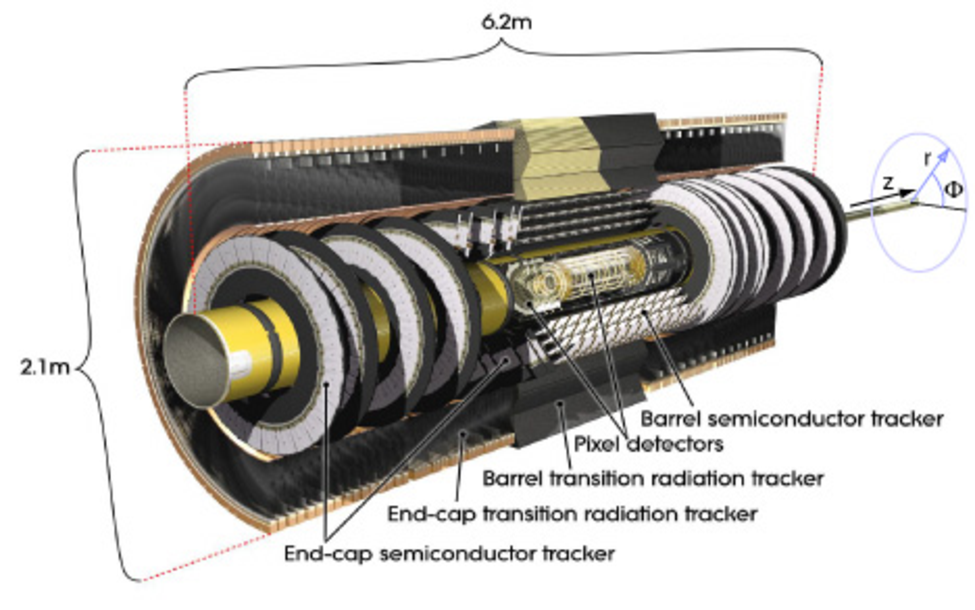
\includegraphics[width=0.8\textwidth]{ATLASDetector/images/innerDetector.pdf}
	\label{fig:inner_detector}  
	\caption{A cutaway picture showing the main components of the ATLAS inner detector.  The ATLAS coordinate system is sketched on the right-hand side of the figure.}
\end{figure}


%http://cds.cern.ch/record/1290332/files/VERTEX%202010_015.pdf
\subsubsection{Pixel System}
\label{sec:pixel}
The pixel system sits physically closest to the beam line and interaction point.  It is built of silicon pixels 
that measure 50 x 400 micrometers each, which are organized into sensors.  Each sensor contains 46,080 
pixels, and then there are 16 sensors organized onto a pixel module.  The pixels as a whole contain 1744 
modules, organized into 3 layers each in the barrel and the two endcaps.  
The pixel system in aggregate contains 80 million channels and measures about 1.4 meters long by 0.4 meters in diameter.

\begin{figure}
	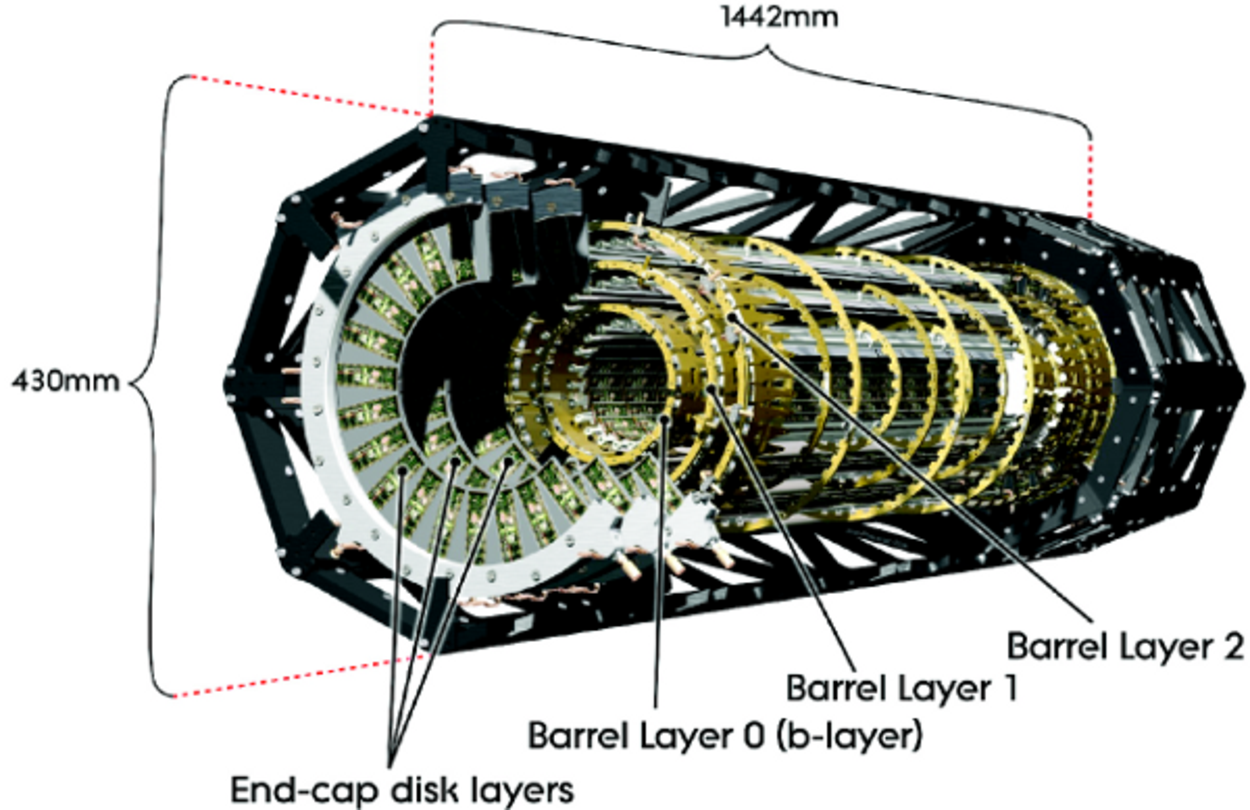
\includegraphics[width=0.8\textwidth]{ATLASDetector/images/pixel_detector.pdf} 
	\caption{A picture showing the main layers of the ATLAS pixel detector, including the disk layers on the end.  Starting in 2015, a 4th layer, the insertable b layer (IBL), will be inserted inside the current layer 0. 	\label{fig:inner_detector} }
\end{figure}

% http://iopscience.iop.org/1748-0221/3/07/P07007/pdf/1748-0221_3_07_P07007.pdf
The pixel technology is designed to give high-precision measurements of the location and momentum of charged tracks.  
A pixel module has two main components, the silicon sensor and the front-end chip, which are 
bump-bonded together.  When a charged particle traverses the sensor it ionizes silicon atoms, creating 
electron-hole pairs, and then a bias voltage applied across the sensor causes the electrons and holes 
to drift to opposite sides of the sensor, where they can be read out by the front-end chips.  

The pixel readout is based on detecting and quantifying this ionization current.  A particle with greater momentum will create 
more electron-hole pairs and thus a longer readout pulse, which passes through a preamplifier and then a 
discriminator.  The discriminator is set with a tunable threshold number of electrons, typically a few thousand, and 
the signal metric is then the length of time for which the pulse was above that value (called ``
time over threshold'', or TOT).  Having a threshold in place helps distinguish ionization current from leakage current, 
which occurs when the silicon does not have robust insulator characteristics and current begins to flow across the sensor even 
when there is no ionizing particle present.  One important effect of radiation damage to the pixel detector is that 
it damages the silicon, allowing for increases in leakage current up to 100 nA, so over the course 
of large radiation doses to the detector the thresholds sometimes have to be raised to compensate for the damaged material.  


%from atlas TDR
\begin{wrapfigure}{R}{0.5\textwidth}
  \begin{center}
%\begin{figure}
	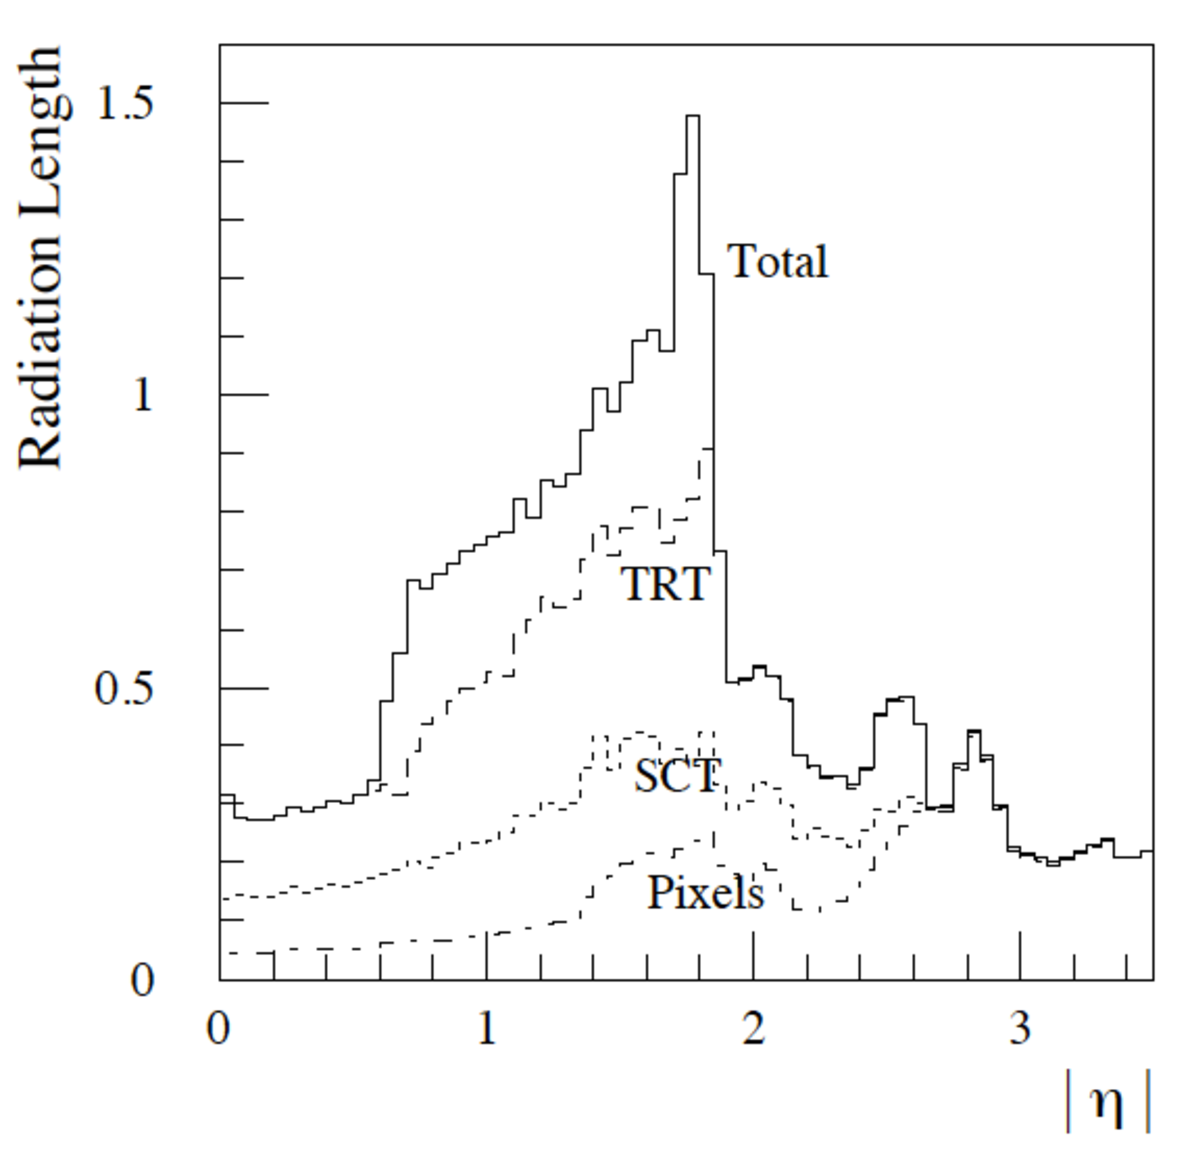
\includegraphics[width=0.45\textwidth]{ATLASDetector/images/id_material_budget.pdf}
	\label{fig:id_material}
	\end{center}
%\end{figure}
\end{wrapfigure}

Another important consideration when designing and constructing the pixel detector is the material budget of the system.  When a 
charged particle traverses the pixels, interacting with the silicon, its trajectory can change by virtue of these interactions 
as it undergoes multiple scattering or secondary interactions.  This can be a problem, for example, when reconstructing 
tracks--if a track has a kink from where it scattered off detector material, it will be more 
challenging to reconstruct the track or correctly measure its momentum.  These material effects are particularly important for the pixel 
detector, because they are the first layer of detector traversed by particles after they leave the collision point.  
One way to mitigate these effects is to place high-material components, such as power supplies and readout 
electronics, in more forward regions so that they are not in the path of central tracks.  There are 
two figures of merit when evaluating the material budget of a system: the radiation length is the distance an 
electromagnetically interacting particle (such as an electron, positron or photon) travels before losing 1/$e$ 
of its energy to bremsstrahlung, while the interaction length is the mean distance traveled by a hadronically-interacting 
particle (such as a proton, neutron or pion) before undergoing an inelastic nuclear interaction.  Figure ~\ref{fig:id_material} 
of the material volume, in units of radiation length vs. $\eta$, shows that the material budget 
(especially pixels) is minimized in the most central regions.


%https://cds.cern.ch/record/1445527/files/ATL-COM-PHYS-2012-471.pdf
The pixel system all together provides fine resolution of the beamspot and surrounding area, which serves several important purposes
.  First, since there are typically many hard p-p collisions in each bunch crossing, the pixels 
system has longitudinal resolution $z_0\sin\theta\approx$0.05-0.3 mm 
enables the reconstruction of multiple primary vertices that are typically separated by a few millimeters \cite{pixel_res}.  This 
is critical for controlling pileup in the high-luminosity LHC environment.  Second, the transverse resolution of 0.01-0.1 mm 
enables the track resolution required to allow precision b-tagging for identification of bottom quarks.  More details
on both the track reconstruction and the $b$-tagging methodology can be found in Sections~\ref{sec:trk_reco} and ~\ref{sec:b-tag}. 


% useful thesis: http://www-pnp.physics.ox.ac.uk/~demirkoz/thesis.pdf
\subsubsection{Semiconductor Tracker (SCT)}
\label{sec:sct}
Like the pixels, the silicon microstrip tracker (SCT) is a silicon detector, although the geometry is 
distinctly different from the pixel geometry.  Since the SCT is at a farther radius from the interaction point than 
the pixels, it experiences a lower occupancy.  This allows for substantially larger detector elements, at a lower 
cost and using less material in the detector than if the same coverage were implemented in pixels, while maintaining 
16 $\mu$m resolution of tracks in r$\Phi$ and 580 $\mu$m resolution in Z ~\cite{sct_res}.   

The SCT geometry has some notable features.  The SCT consists of 8 layers of microstrips organized into 4 double
-sided pairs, where the two members of each pair have an offset angle of 40 mrad.  The 
SCT has 4 barrel layers and 9 endcap disks, and the barrel modules are oriented with a tilt angle 
of about 11$^\circ$ angle relative to being perfectly tangential to $r\phi$ ~\cite{tdr}.  Whereas the 
pixel reads out the TOT of a hit, the SCT has a binary readout: a hit is either recorded or not.



%https://indico.cern.ch/getFile.py/access?contribId=51&sessionId=8&resId=0&materialId=slides&confId=117804
\subsubsection{Transition Radiation Tracker}
\label{sec:trt}
The outermost inner detector layer is the transition radiation tracker, or TRT.  

The TRT uses gold-plated tungsten wires embedded in straw tubes of 4mm diameter filled with an Xe/O$_2$/Co$_2$ 
gas mixture, with a total of about 350,000 readout channels covering a pseudorapidity range out to $|\eta|<$2.0.
  For a typical particle, the TRT will have about 30-35 hits with a hit precision of about 130$\mu m$ ~\cite{trt}.

One important objective of the TRT is to identify tracks from electrons by detecting transition radiation (hence the name 
transition radiation tracker).  Transition radiation occurs when an electron passes between regions with different 
dielectric constants; at the boundary between those regions, the electron can emit a photon which is then absorbed 
by the Xe gas and translates into a high-threshold hit in the detector.  Electrons can be distinguished 
from hadrons by the presence of many high threshold hits along the track.

 


\subsection{Calorimeters}
The ATLAS calorimeters measure the energy of particles.  There are two main calorimeter
subsystems, one for electromagnetic particles and the other for hadronically-decaying particles.
In addition to energy measurements, though, information from the calorimeters also is used
for particle identification, finding the direction of electromagnetic and hadronic jets, 
identifying and measuring missing transverse energy or MET, and selecting jets as part of the
trigger.



The ATLAS detector has two calorimeter systems: the electromagnetic (EM) calorimeter, designed to measure the energy 
of electrons and photons, and the hadronic calorimeter, for measuring the energy of hadrons, jets, tau 
leptons and missing transverse energy.  

%http://www-library.desy.de/preparch/desy/proc/proc10-01/meng.pdf
%http://iopscience.iop.org/1742-6596/110/9/092007/pdf/jpconf8_110_092007.pdf
\subsubsection{Electromagnetic Calorimeter}
\label{sec:em_cal}

The electromagnetic (EM) calorimeter measures electrons and photons after they exit the tracking system. It was
designed with the discovery of the SM Higgs boson in mind, since for many possible values of $m_h$ (including 
the value where the particle was actually found, $m_h$=126 GeV), the most sensitive search channels contain 
electromagnetic particles (electrons and photons) in the final state. 

Nicknamed the LAr 
calorimeter for its liquid argon technology,  the calorimeter is a sampling calorimeter, with the passive showering material (
lead) interleaved with active energy measurement material (liquid argon).  An electron or photon will interact with the 
lead as it travels through it, creating an electromagnetic shower, which then propagates to the adjacent LAr layer
, where it is measured and read out.


\begin{figure}
\begin{center}
	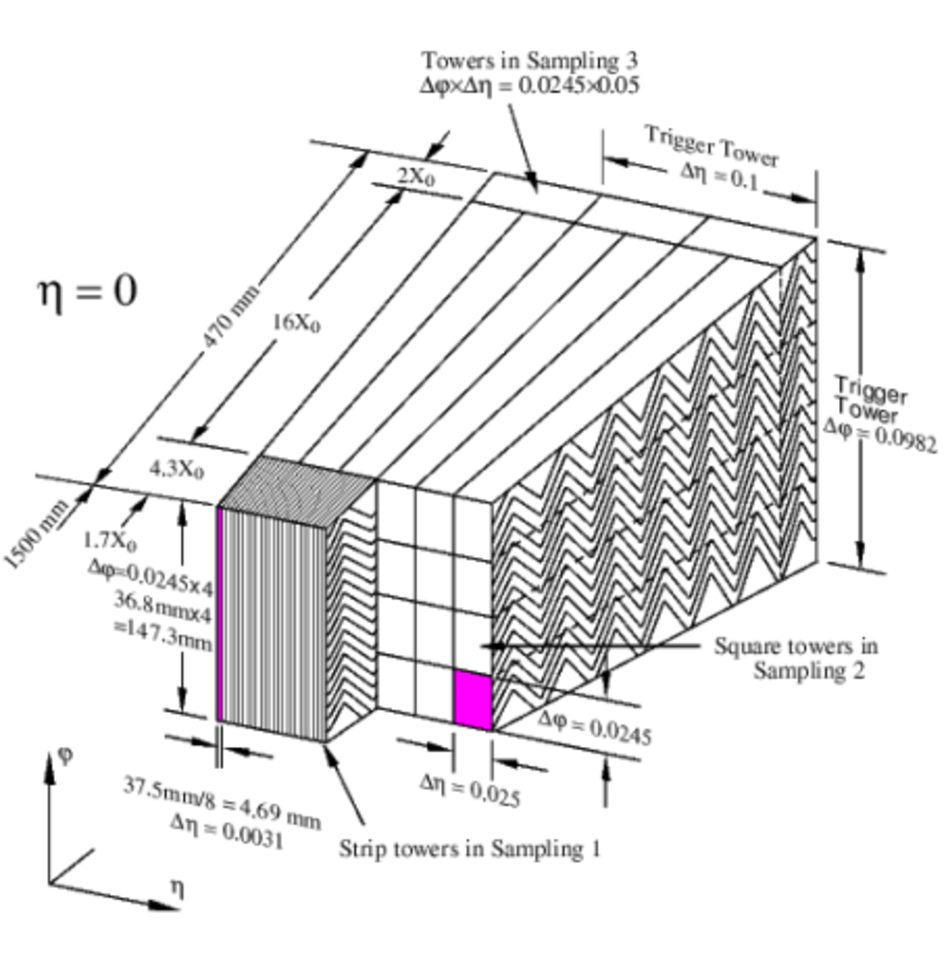
\includegraphics[width=0.6\textwidth]{ATLASDetector/images/LArg_accordion.pdf}	
	\caption{A depiction of a section of the LAr calorimeter.  The accordion structure of the towers is visible, as well as the three sampling layers. 	\label{fig:lar}}
\end{center}
\end{figure}


A notable feature of the EM calorimeter is the accordion geometry, which has several key characteristics.  First, 
the geometry enables complete coverage in $\phi$ without azimuthal cracks.  Second, the LAr sampling layer between 
lead layers is constant throughout the calorimeter barrel.  Third, a particle traveling through the calorimeter will generate approximately 
the same number of sampling instances (i.e. measurements) regardless of the direction in which it 
travels.  These pieces add up to a very uniform coverage of electromagnetic calorimetry.  The calorimeter consists of two 
major parts, the barrel and the endcaps; the barrel measures particles with $|\eta|<$1.475 
and the endcaps measure particles with 1.375$<|\eta|<$3.2.  The transverse segmentation of the calorimeter
is $\Delta\eta \times \Delta\phi<$0.03$\times$ 0.03 over the pseudorapidity region $|\eta|<$2.5,  
to allow for the particle identification and energy resolution needed \cite{cal_tdr}, while the 
calorimeter is up to 24 radiation lengths thick to minimize punch-through.

The performance requirement for the energy resolution of the EM calorimeter is 
$\sigma_E/E=\frac{10\%}{\sqrt{E}}+$0.7\%, which has the nice feature that the resolution improves
as the energy of an electromagnetic jet increases.
A crucial part of reaching this resolution is precisely understanding the shape of the readout pulse.  The traversing particle 
produces an electromagnetic shower where the drift time of the particles in the shower cause a readout pulse that is 
roughly triangular in shape and typically 400 ns long.  This pulse is shaped by the readout electronics and the 
signal shape is simulated with Monte Carlo and calibrated using precisely known test pulses deposited into the readout chain.  
However, as detailed below, the presence of multiple interactions per bunch crossing, known as pileup, has 
a significant effect in the calorimeters and is an important task for understanding jet energy.

%http://cds.cern.ch/record/1478440/files/ATL-TILECAL-PROC-2012-008.pdf
%http://arxiv.org/pdf/1305.0550v1.pdf
%http://cds.cern.ch/record/1393742/files/CERN-THESIS-2011-144.pdf
\subsubsection{Hadronic Calorimeter} 
\label{sec:h_cal}
Like the EM calorimeter, the hadronic calorimeter was designed with an eye toward Higgs discovery, that it would
have the resolution needed to find Higgs decays to $b\bar{b}$ and $\tau\tau$ pairs.  This is important and complementary
to the EM calorimeter because, although the most sensitive decay channels of the Higgs are to photons and electrons,
the decay modes with the highest branching fractions ($b\bar{b}$ and a large subset of $W^+W^-$) are hadronic.
For the physics in this thesis, with three $b$-jets in the final state, the hadronic calorimeter does the crucial
jet energy detection and measurement. 

Accurate measurement of hadronic energy is crucial for accurately reconstructing $b$-jets, and the hadronic calorimeter also measures the 
energy from hadrons, jets, taus and allows for a measurement of missing transverse energy.  The hadronic calorimeter 
is a sampling calorimeter, nicknamed the tile calorimeter because of its composition of scintillating tiles (active material) 
interleaved with steel plates (showering material) in the barrel.  When a strongly-interacting particle hits the steel it creates a 
spray of particles, called a shower, which then enters the scintillator and creates a light signal that is 
proportional to the energy .  This process repeats until the full energy of the original particle is measured, and 
usually the calorimeter cells are reconstructed into an object called a jet which aims to cluster the energy together in 
a way that accurately represents the energy of the original particle.  Much more on hadronic jet reconstruction will follow in Section~\ref{sec:jet_reco}.

The hadronic calorimeter is partitioned into four major subsections, two barrel sections and two extended barrel sections, allowing 
for measurements out to $|\eta|<$1.7.  In the forward regions, hadronic coverage is provided by the liquid argon system and the high-density forward calorimeter \cite{cal_tdr}. In order to stop all remaining particles from the collision, 
with the notable exception of muons, the hadronic calorimeter is about 7.4 radiation lengths ($\lambda$) thick.

\begin{figure}
	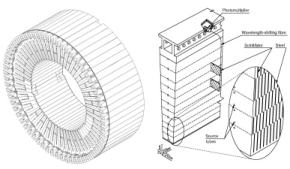
\includegraphics[width=0.8\textwidth]{ATLASDetector/images/tile_cal.pdf}
	\caption{A depiction of the scintillator-and-steel hadronic calorimeter, also known as the tile calorimeter, and a close-up view of one of its cells.	\label{fig:tile_cal}}
\end{figure}


%http://iopscience.iop.org/1742-6596/331/2/022024/pdf/1742-6596_331_2_022024.pdf

\subsection{Muon System}
\label{sec:ms}
Muons are very similar to electrons in their interactions, but they are about 200 times heavier and as a 
result, they can travel largely unaffected through the inner detector and calorimeters and emerge in the outer layers of 
the detector, where the muon system is situated to make dedicated measurements of muons.  The muon system is 
often used in conjunction with the tracking of the inner detector, since a muon interacts electromagnetically and would be 
expected to create a track in both systems.  These tracks in the two different subsystems can then be combined 
into a single measurement of the $p_T$ of the muon.  Muons are largely not used 
in this analysis, so we will be brief in explaining the muon system, although they may play an 
important role in the future since muons can be used to help trigger on and identify $b$-jets.


The ATLAS muon system is composed of four different detector systems located within and around an air-core toroid 
magnet with a field of 1 Tesla.  Precision tracking in the barrel is done by Monitored Drift Tubes (
MDT) and in the endcap by Cathode Strip Chambers (CSC).  Quick-readout triggering is done in 
the barrel by Resistive Plate Chambers (RPC) and in the endcap by Thin Gap Chambers (TGC).   
The system is designed to measure the $p_T$ of muons with $p_T>$
3 GeV, with 3\% resolution up to $p_T<$250 GeV and 10\% resolution up to 1TeV.  



%%% ATLAS detector figure
\begin{figure}
	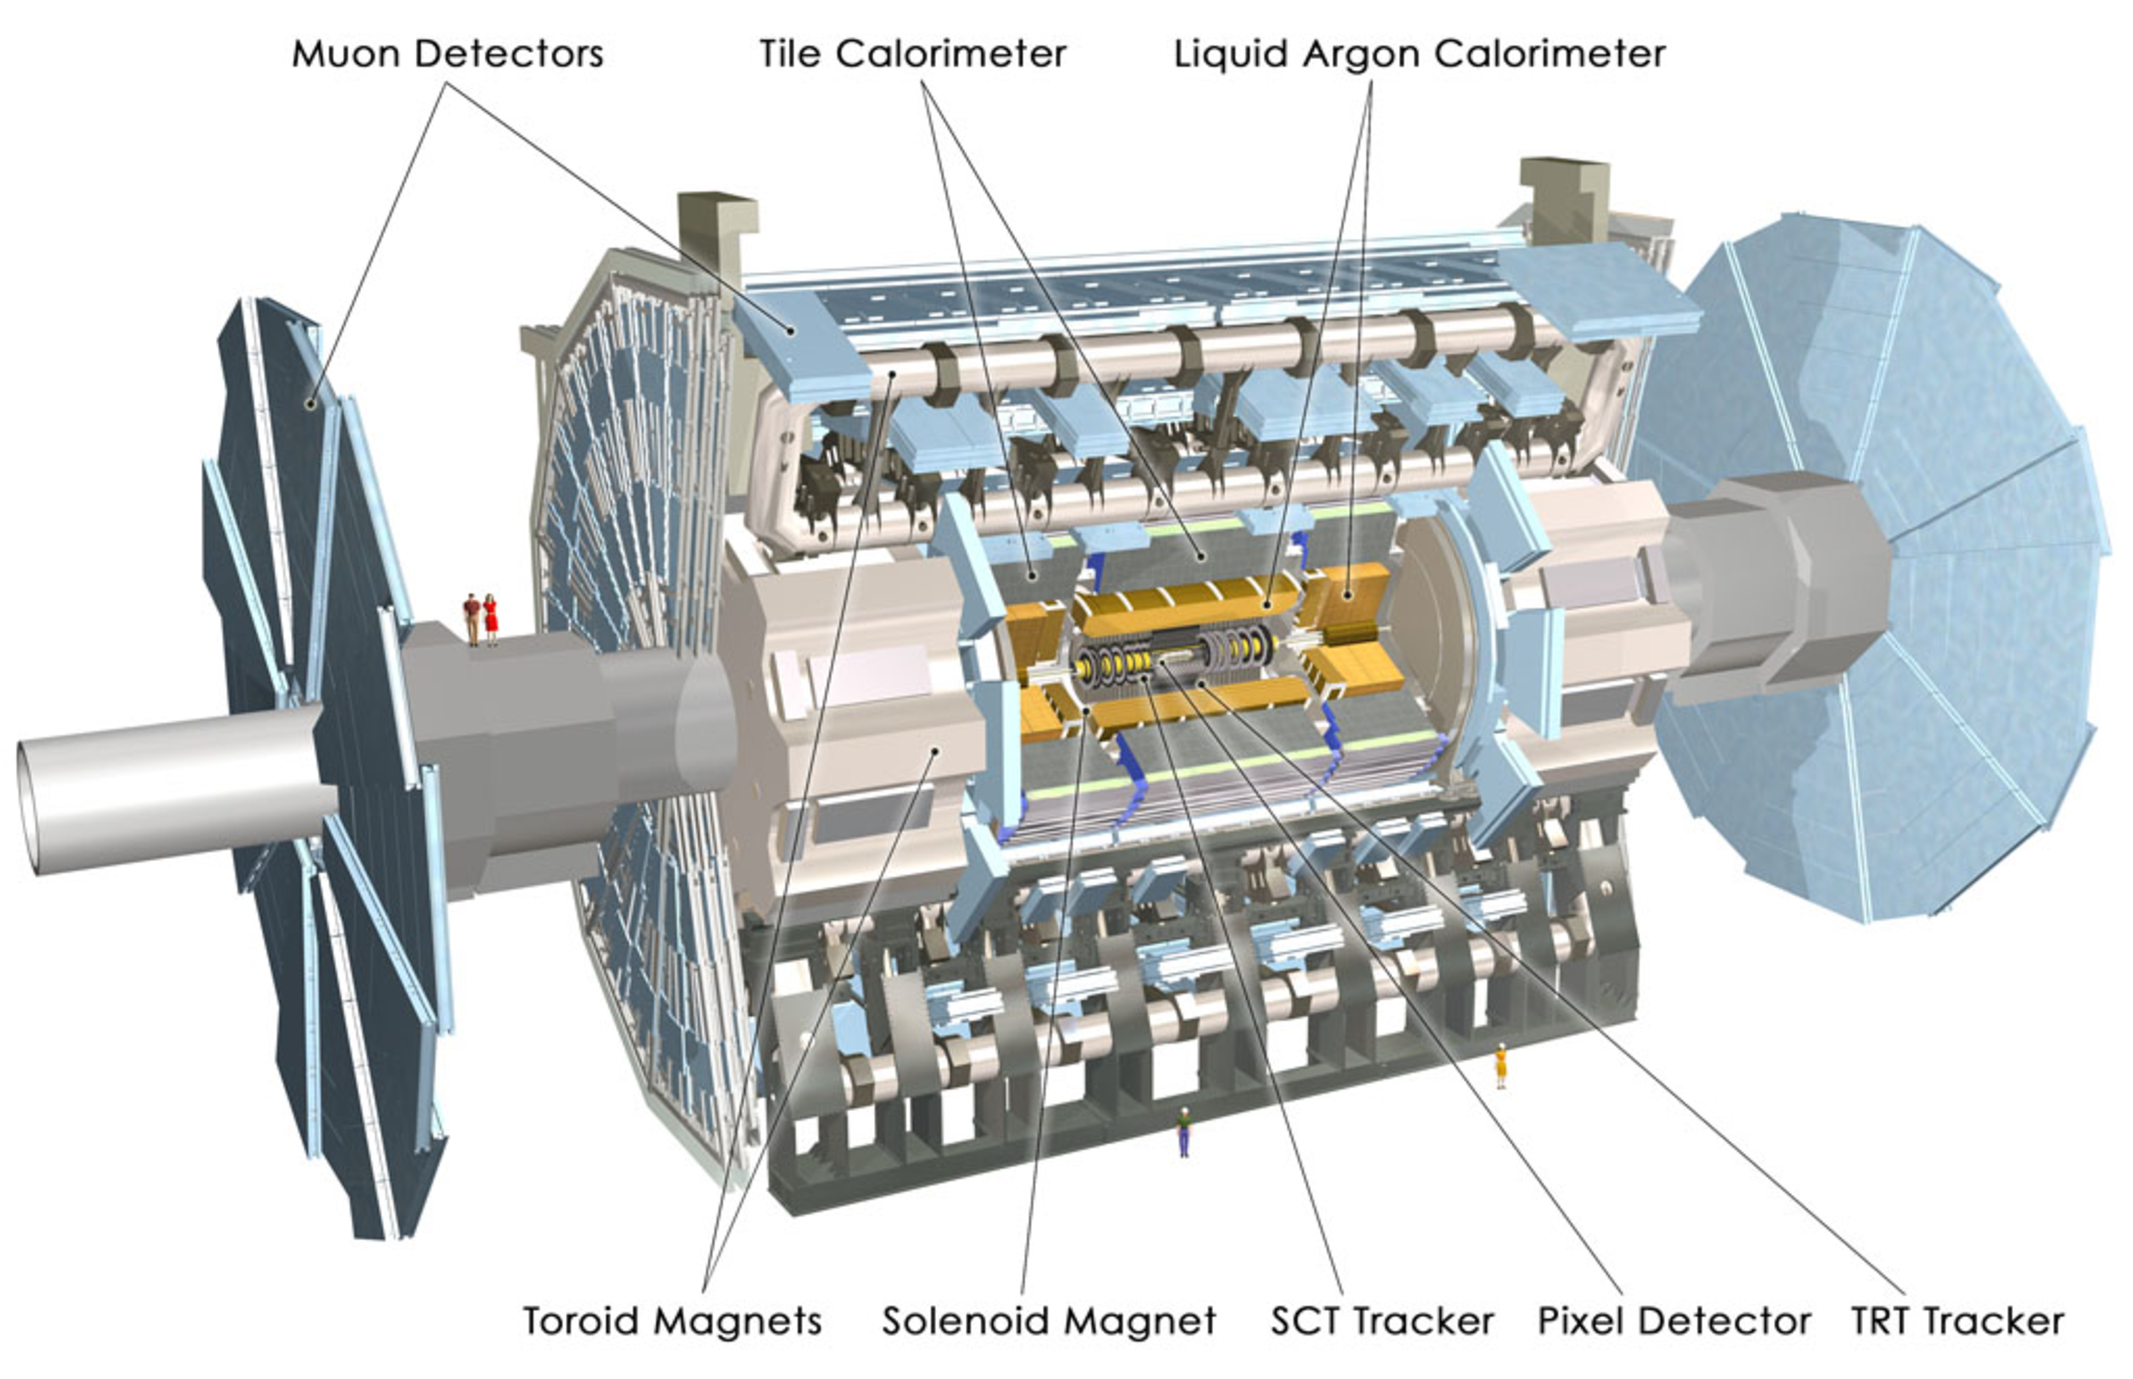
\includegraphics[width=\textwidth]{ATLASDetector/images/AtlasDetectorLabeled.pdf}	\caption{A diagram of the ATLAS detector as a whole, with major subsystems labeled.  A couple of human figures are shown standing on and near the detector, for scale. \label{fig:detector}}
\end{figure}

%http://www.slac.stanford.edu/econf/C0303241/proc/pres/502.PDF
%https://cds.cern.ch/record/1267390/files/ATL-DAQ-SLIDE-2010-087.pdf
\section{The ATLAS Trigger and Data Processing}
\label{sec:atlas_trig}
Although the LHC delivers 20 million bunch crossings per second to the ATLAS detector, the detector does not have 
the capacity in either storage space or readout bandwidth to record all these collisions.  The trigger has the task 
of selecting the most interesting 200 or so events per second, which are then fully reconstructed and recorded.  
The trigger is a three-layer system, with a first level (L1) implemented solely in hardware
, a second level (L2) that reconstructs ``regions of interest'' (RoIs) with special fast 
algorithms, and an event filter (EF) that reconstructs the full event with offline algorithms.  L2 and 
EF together are called the high level trigger, or HLT.

In what follows, we will make use of the following terminology in explaining the structure and performance of the trigger:

\begin{itemize}
	\item trigger object: the signature left by a particle in the detector, once it has been reconstructed and identified.  Examples include electrons, muons, photons, and jets.
	\item trigger item: one or more trigger objects that define whether an event passes a particular level (L1, L2, EF)
	\item threshold: the minimum momentum or energy required in order for a trigger object to be accepted.
	\item trigger accept: when all the requirements for a particular trigger level are met, and the event gets promoted to the next level.

	\item trigger chain: a set of L1, L2 and EF trigger items (also called simply a trigger).
	\item trigger menu: the set of all L1, L2 and EF trigger items, which collectively define which events will be written to disk.
	\item trigger prescale: a set reduction factor, so that a trigger can be maintained with low thresholds while not exceeding rate limits.  For example, for a trigger with a prescale of 10, only 1 in 10 events passing the trigger get written to disk.
\end{itemize}
 

The trigger has a step-type structure, where progressively smaller numbers of events are processed with progressively more 
detailed and computationally intensive algorithms.  Many physics analyses look for signatures that have more than one physics object in 
them (for instance, multiple electrons, or a lepton plus jets), so multiple physics objects are often 
required in a single trigger.  There are also single-item triggers, although typically these have higher thresholds 
than triggers that look for multiple objects.  If all of the objects in a given trigger item are seen
, the event is accepted for the current level and the event moves forward in the data collection process.  
This process repeats three times, once for each of the levels of the trigger--only those events which 
pass L1 move onto L2, those which pass L2 move on to EF, and those that pass EF 
are written to disk.   As the machine settings for the LHC changed over the course of 2012, resulting 
in different conditions for data-taking, the trigger menu was adjusted periodically to keep rates under control (
in practice, this generally means either raising thresholds or adding prescales).  


Groups of trigger chains that share common features are grouped together into trigger streams, where the primary trigger streams 
are JetTauEtMiss, EGamma, MinBias, and CosmicCalo.  The end result of this process is approximately 200 events 
per second (320 GB/s of data) being written to disk; the trigger rates and latency 
information can be found in Table \ref{tab:trigger_stats}.

  

% https://cds.cern.ch/record/1181075/files/05446486.pdf
\begin{table}
\begin{tabular}{c | c | c | c}
Trigger Level & Rate in Hz  & Latency  & Data Rate\\  \hline
None (Event rate) & 20 MHz  & no decision applied yet & 1600 TB/s \\
L1  & 75 kHz  &  $\sim$ 1$\mu s$  & 120 GB/s\\
L2  & 3 kHz    & $\sim$ 10 ms & 5 GB/s \\
EF  &  200 Hz  & $\sim$ 1 s & 320 MB/s \\
\end{tabular}
\end{table}
\label{tab:trigger_stats}


Of particular interest to this analysis are the jet thresholds and b-tagging applied in the trigger.  This 
will be outlined in greater detail in a later section, but we will introduce the ideas here.  As 
only 200 events per second get written to disk, the bandwidth has to be carefully allocated across triggers, 
and it is very expensive to keep a trigger that allows high rates of events to be written to data
.  In an analysis such as this one, the physics objects coming from the signal (b-jets 
from a Higgs decay) are generally higher in p$_T$ than the background (continuum QCD processes
) so one way to keep event rates reasonable in the face of rising luminosity is to place higher p$_T$ 
thresholds on the jets that fire the trigger.   

The thresholds increase with each trigger level, as more information is read out of the detector, so that 
a jet which is reconstructed with 145 GeV of p$_T$ at L1 
might be required to have 155 GeV at EF in order to pass the full trigger.  Once the event 
is written to disk, it is subject to the full offline reconstruction and calibration so that the final p$_T$ 
of the jet might not be exactly the number measured at the trigger EF.  There is therefore a range 
of p$_T$ values, called the turn-on curve, where the trigger goes from rejecting 
all events to accepting all events.  Within the turn-on curve even a small change in the p$_T$
of a jet can have a dramatic difference in whether the jet fires a trigger accept, so this 
instability is mitigated by placing p$_T$ cuts on the trigger jets that require that their respective p$_T$ 
values are above the turn-on curve.  

The ATLAS trigger also allows for b-tagging of jets at L2 and EF.  For analyses that have 
b-jets in the final state, b-tagging in the trigger provides a tool for keeping rates 
low without pushing up jet p$_T$ thresholds.  B-tagging in the trigger introduces several challenges
, though.  First, the online b-tagging algorithms have less time and information than the offline algorithms
.  Second, a jet that passes an L2 b-tag will not necessarily pass an EF b-
tag, and vice versa, so more work is required in understanding the correlations between tags at different trigger 
levels.  







